\usepackage[
  paperwidth=170mm,
  paperheight=240mm,
  inner=20mm,
  outer=17mm,
  top=20mm,
  bottom=22mm,
  headheight=14pt,
  headsep=7mm
]{geometry}

\usepackage{fontspec}
\IfFileExists{font/times.ttf}{
  \setmainfont{times.ttf}[
    Path=font/,
    BoldFont=timesbd.ttf,
    ItalicFont=timesi.ttf,
    BoldItalicFont=timesbi.ttf
  ]
}{
  \setmainfont{texgyrepagella-regular.otf}[
    BoldFont=texgyrepagella-bold.otf,
    ItalicFont=texgyrepagella-italic.otf,
    BoldItalicFont=texgyrepagella-bolditalic.otf
  ]
}

\setsansfont{texgyreheros-regular.otf}[
  BoldFont=texgyreheros-bold.otf,
  ItalicFont=texgyreheros-italic.otf,
  BoldItalicFont=texgyreheros-bolditalic.otf
]
\setmonofont{texgyrecursor-regular.otf}[
  BoldFont=texgyrecursor-bold.otf,
  ItalicFont=texgyrecursor-italic.otf,
  BoldItalicFont=texgyrecursor-bolditalic.otf
]

\IfFileExists{font/simsun.ttc}{
  \setCJKmainfont{simsun.ttc}[
    Path=font/,
    FontIndex=0,
    BoldFont=simhei.ttf,
    ItalicFont=simkai.ttf,
    BoldItalicFont=simhei.ttf
  ]
  \setCJKsansfont{simhei.ttf}[
    Path=font/,
    BoldFont=simhei.ttf
  ]
  \setCJKmonofont{simsun.ttc}[
    Path=font/,
    FontIndex=1
  ]
}{
  \setCJKmainfont{FandolSong-Regular.otf}[
    BoldFont=FandolSong-Bold.otf,
    ItalicFont=FandolKai-Regular.otf
  ]
  \setCJKsansfont{FandolHei-Regular.otf}[
    BoldFont=FandolHei-Bold.otf
  ]
  \setCJKmonofont{FandolFang-Regular.otf}
}

\usepackage{xcolor}
\definecolor{AgentInk}{HTML}{1D2730}
\definecolor{AgentGreen}{HTML}{14866D}
\definecolor{AgentBlue}{HTML}{2B6F9C}
\definecolor{AgentGold}{HTML}{D89B32}
\definecolor{AgentCoral}{HTML}{CF5A5A}
\definecolor{CoverRed}{HTML}{D94F35}
\definecolor{AgentMist}{HTML}{F1F5F3}
\definecolor{AgentPaper}{HTML}{FCFDFC}
\definecolor{AgentLine}{HTML}{D6E0DC}
\definecolor{CodeBg}{HTML}{F5F7F6}

\pagecolor{AgentPaper}
\color{AgentInk}

\usepackage{microtype}
\usepackage{setspace}
\setstretch{1.16}
\setlength{\parindent}{2em}
\setlength{\parskip}{0.25em}

\usepackage{graphicx}
\usepackage{tikz}
\usetikzlibrary{arrows.meta,calc,fit,positioning,shapes.geometric}
\usepackage{booktabs}
\usepackage{tabularx}
\usepackage{longtable}
\usepackage{array}
\usepackage{enumitem}
\setlist{nosep,leftmargin=2em}
\setlist[itemize]{label=\textcolor{AgentGreen}{\small\textbullet}}
\setlist[enumerate]{label=\textcolor{AgentBlue}{\arabic*.}}

\usepackage{titlesec}
\titleformat{\part}[display]
  {\centering\sffamily\bfseries\color{AgentGreen}}
  {\fontsize{18}{22}\selectfont 第\thepart\ 部分}
  {1.1em}
  {\fontsize{32}{38}\selectfont}

\titleformat{\chapter}[display]
  {\sffamily\bfseries\color{AgentInk}}
  {\color{AgentGreen}\fontsize{13}{16}\selectfont CHAPTER\enspace\thechapter}
  {0.6em}
  {\fontsize{27}{33}\selectfont}
  [\vspace{0.7em}\color{AgentLine}\titlerule]

\titleformat{\section}
  {\Large\sffamily\bfseries\color{AgentBlue}}
  {\thesection}{0.65em}{}
\titleformat{\subsection}
  {\large\sffamily\bfseries\color{AgentGreen}}
  {\thesubsection}{0.6em}{}

\titlespacing*{\chapter}{0pt}{-12pt}{24pt}
\titlespacing*{\section}{0pt}{1.8em}{0.7em}
\titlespacing*{\subsection}{0pt}{1.4em}{0.5em}

\usepackage{fancyhdr}
\pagestyle{fancy}
\fancyhf{}
\fancyhead[LE]{\small\sffamily\color{AgentGreen}\thepage\quad 动手学 Agent}
\fancyhead[RO]{\small\sffamily\color{AgentGreen}\leftmark\quad\thepage}
\renewcommand{\headrulewidth}{0pt}
\fancypagestyle{plain}{
  \fancyhf{}
  \fancyfoot[C]{\small\sffamily\color{AgentGreen}\thepage}
  \renewcommand{\headrulewidth}{0pt}
}

\usepackage[most]{tcolorbox}
\tcbset{
  enhanced,
  boxrule=0.6pt,
  arc=1.5mm,
  left=3.2mm,
  right=3.2mm,
  top=2.4mm,
  bottom=2.4mm,
  before skip=1em,
  after skip=1em,
  fonttitle=\sffamily\bfseries
}

\newtcolorbox{definitionbox}[1]{
  title={#1},
  colback=AgentMist,
  colframe=AgentGreen,
  coltitle=AgentGreen
}
\newtcolorbox{takeaway}[1][本节要点]{
  title={#1},
  colback=AgentMist,
  colframe=AgentBlue,
  coltitle=AgentBlue
}
\newtcolorbox{practice}[1][动手任务]{
  title={#1},
  colback=AgentGold!7,
  colframe=AgentGold,
  coltitle=AgentInk
}
\newtcolorbox{warningbox}[1][风险提示]{
  title={#1},
  colback=AgentCoral!6,
  colframe=AgentCoral,
  coltitle=AgentCoral
}
\newtcolorbox{checkpoint}[1][完成检查]{
  title={#1},
  colback=AgentGreen!5,
  colframe=AgentGreen,
  coltitle=AgentGreen
}

\usepackage{fvextra}
\DefineVerbatimEnvironment{codeblock}{Verbatim}{
  fontsize=\small,
  breaklines=true,
  breakanywhere=true,
  frame=single,
  rulecolor=\color{AgentLine},
  framesep=3mm
}

\newcommand{\code}[1]{\texttt{\small #1}}
\newcommand{\term}[1]{\textbf{\color{AgentGreen}#1}}
\newcommand{\eng}[1]{\textsf{#1}}
\newcommand{\checkbox}{\raisebox{0.15ex}{\tikz\draw[AgentGreen,line width=0.5pt] (0,0) rectangle (0.16,0.16);}\,}

\usepackage{natbib}
\bibliographystyle{plainnat}
\setcitestyle{numbers,square,comma}

\usepackage{xurl}
\usepackage{hyperref}
\hypersetup{
  hypertexnames=false,
  colorlinks=true,
  linkcolor=AgentGreen,
  citecolor=AgentBlue,
  urlcolor=AgentBlue,
  pdfauthor={DreamingRiverForUs},
  pdftitle={动手学 Agent},
  pdfsubject={AI Agent 实践电子书},
  pdfkeywords={AI Agent, LLM, MCP, RAG, Evaluation}
}
\urlstyle{same}
\usepackage{bookmark}

\newcommand{\BookVersion}{0.1.0-draft}
\newcommand{\BookDate}{2026-08-31}

\newcommand{\makedigitalcover}{
  \begin{titlepage}
    \pagecolor{AgentPaper}\color{AgentInk}
    \begin{tikzpicture}[remember picture,overlay]
      \node[inner sep=0pt] at (current page.center) {
        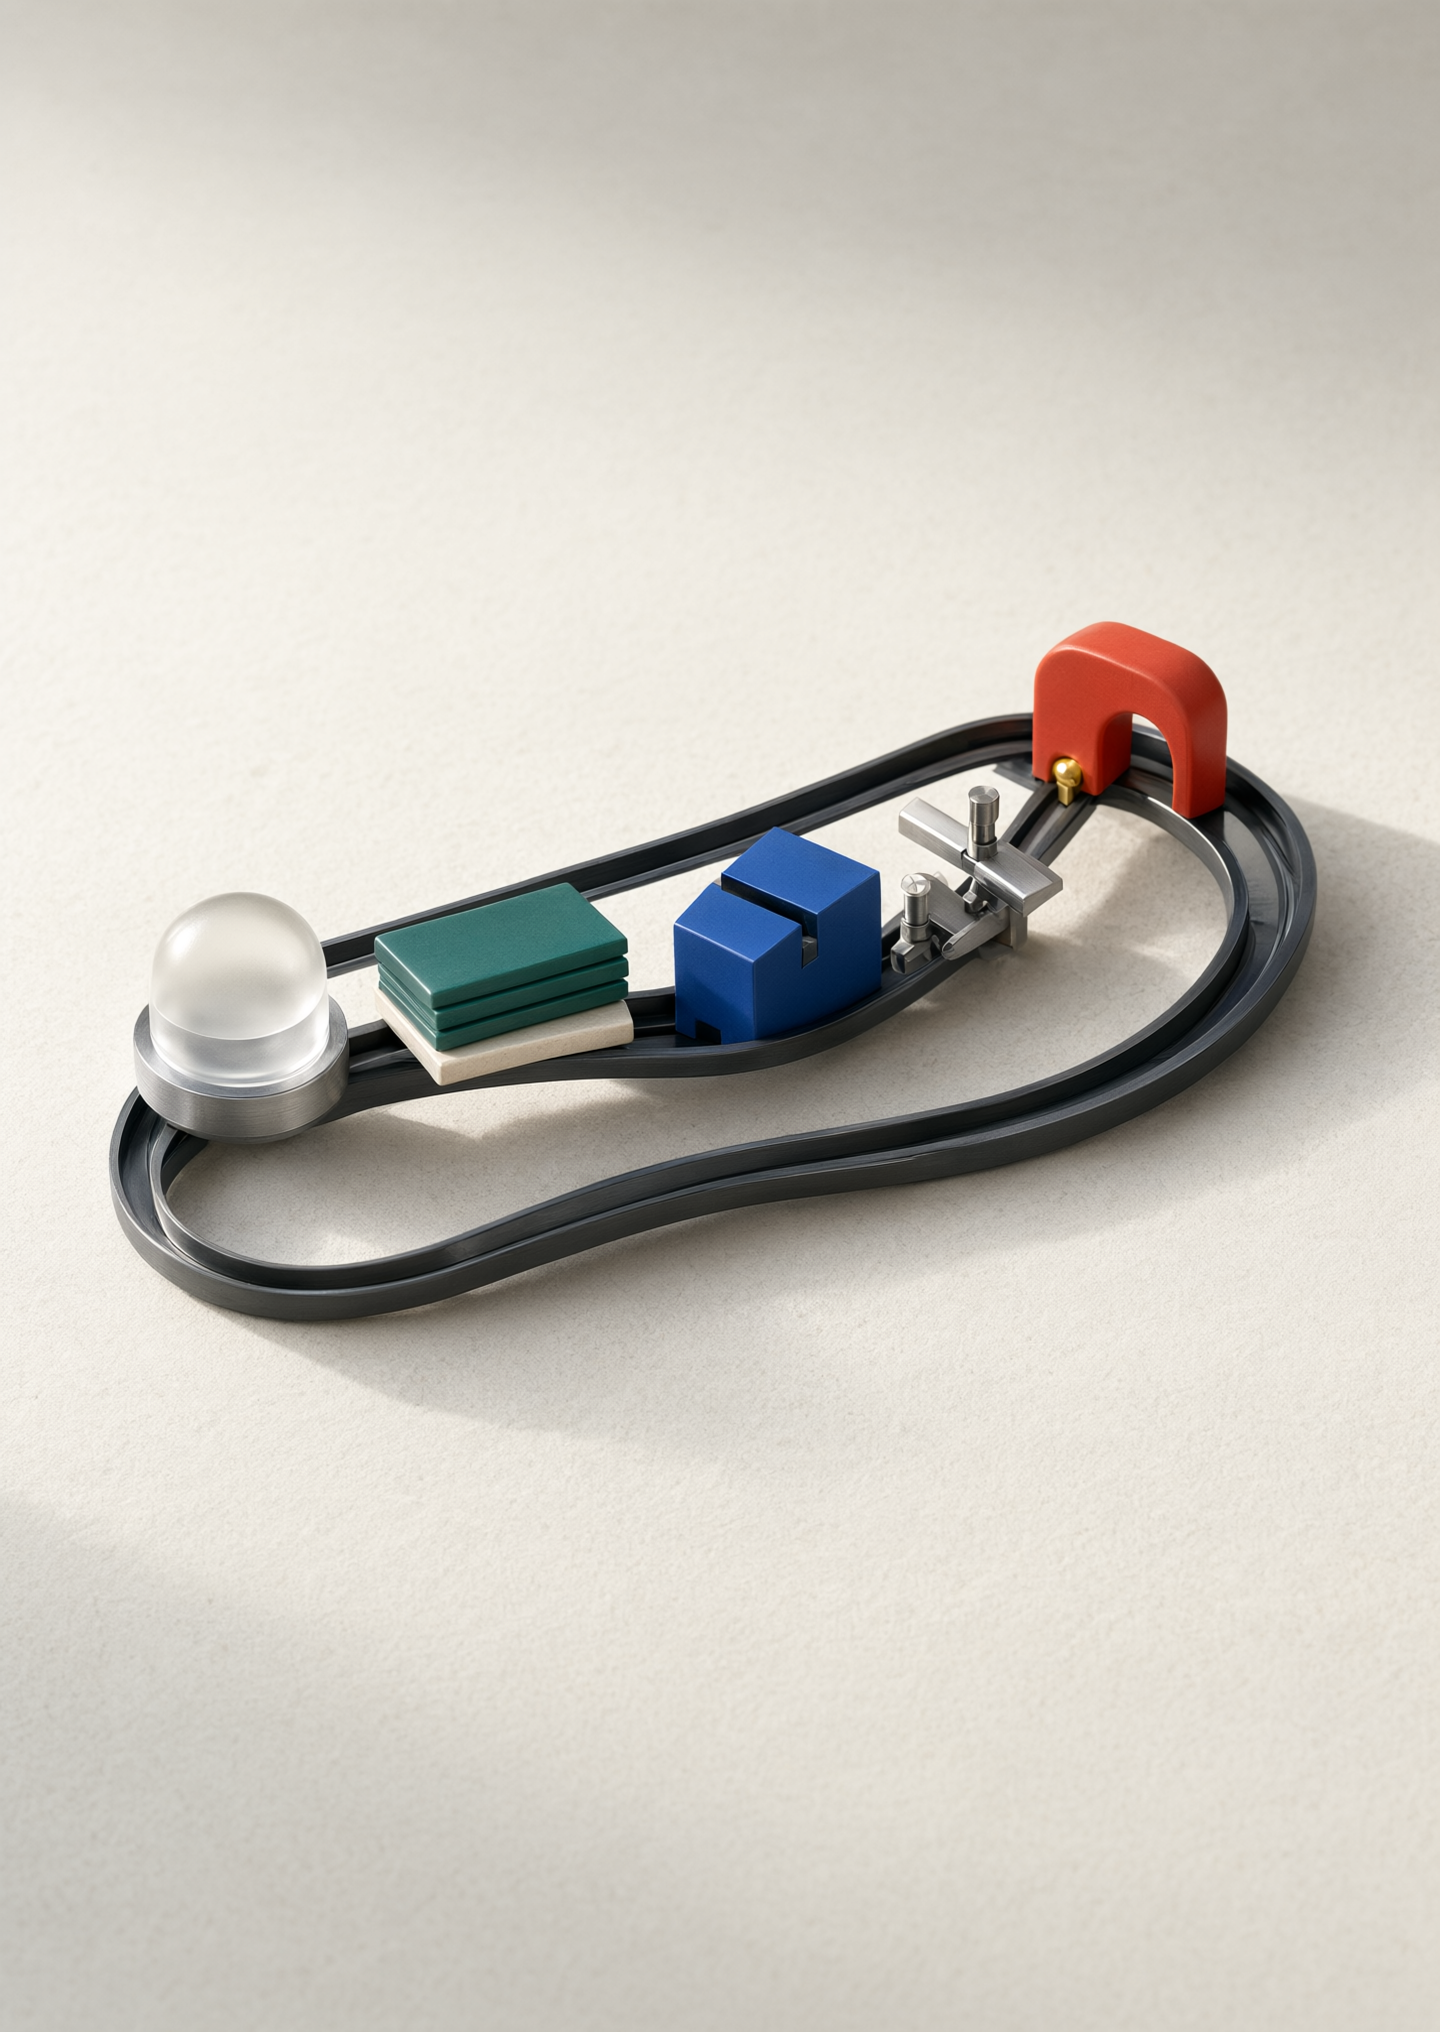
\includegraphics[width=\paperwidth,height=\paperheight]{assets/cover/cover-art-01.png}
      };
    \end{tikzpicture}

    \vspace*{4mm}
    {\sffamily\fontsize{9.5}{12}\selectfont\bfseries\color{AgentBlue}
      PRACTICAL AI SYSTEMS\par}
    \vspace{5mm}
    {\sffamily\bfseries\fontsize{43}{51}\selectfont
      动手学\enspace\textcolor{CoverRed}{Agent}\par}
    \vspace{3mm}
    {\sffamily\fontsize{15}{20}\selectfont 从最小循环到生产级智能体系统}\par
    \vspace{4mm}
    {\color{AgentInk!55}\rule{31mm}{0.7pt}}\par

    \vfill
    {\sffamily\small\bfseries DreamingRiverForUs}\hfill
    {\sffamily\small v\BookVersion}
    \vspace*{6mm}
  \end{titlepage}
  \pagecolor{AgentPaper}\color{AgentInk}
}
